% !TEX program = xelatex
\documentclass[12pt,a4paper]{article}

\usepackage{fontspec}
\usepackage{polyglossia}
\setmainlanguage{greek}
\setotherlanguage{english}
\setmainfont[Script=Greek]{DejaVu Serif}
\setsansfont[Script=Greek]{DejaVu Sans}
\setmonofont[Script=Greek]{DejaVu Sans Mono}
\newfontfamily\greekfonttt[Script=Greek]{DejaVu Sans Mono}

\usepackage[a4paper, margin=2.45cm]{geometry}
\usepackage{amsmath, amssymb}
\usepackage{booktabs}
\usepackage{array}
\usepackage{graphicx}
\usepackage{float}
\usepackage{caption}
\usepackage[hidelinks]{hyperref}
\usepackage{enumitem}
\usepackage{parskip}
\usepackage{xcolor}
\usepackage{listings}
\usepackage{fancyhdr}

\pagestyle{fancy}
\fancyhf{}
\lhead{4η Εργασία -- Explanatory Report}
\rhead{Ερώτημα 1}
\cfoot{\thepage}
\setlength{\headheight}{14.5pt}

\newcommand{\code}[1]{\texttt{\textenglish{#1}}}

\lstset{
    basicstyle=\ttfamily\small,
    breaklines=true,
    frame=single,
    backgroundcolor=\color{gray!8},
    columns=fullflexible,
    keepspaces=true
}

\title{
    \textbf{Ανάλυση Δεδομένων 2025--26}\\[0.25cm]
    \Large 4η Εργασία -- Explanatory Report\\[0.15cm]
    \large Ερώτημα 1: Δέντρο ταξινόμησης μέγιστου βάθους 2
}
\author{
    Ρακοβαλής Παύλος\\
    ΑΕΜ: 6931
}
\date{\today}

\begin{document}

\maketitle
\thispagestyle{fancy}

\begin{abstract}
Το παρόν κείμενο είναι ένα επεξηγηματικό report για το πρώτο ερώτημα της
4ης εργασίας. Είναι γραμμένο σαν να απευθύνεται σε αναγνώστη που δεν έχει
προηγούμενη εμπειρία στην Ανάλυση Δεδομένων. Για αυτόν τον λόγο, πριν από τη
λύση εξηγούνται έννοιες όπως μεταβλητή στόχος, προβλεπτικές μεταβλητές,
training set, test set, δέντρο ταξινόμησης, μέγιστο βάθος δέντρου, accuracy
και confusion matrix. Στο τέλος παρουσιάζεται αναλυτικά η λύση του ερωτήματος
και ερμηνεύονται τα αποτελέσματα.
\end{abstract}

\tableofcontents
\newpage

%=============================================================================
\section{Το ερώτημα της εργασίας}
%=============================================================================

Το πρώτο ερώτημα της 4ης εργασίας είναι:

\begin{quote}
\textbf{«Να γίνει πρόβλεψη/εκτίμηση του τύπου κρασιού με δέντρο ταξινόμησης
μέγιστου βάθους 2 (max depth).»}
\end{quote}

Με πιο απλά λόγια, η εργασία μάς ζητάει να φτιάξουμε ένα μοντέλο το οποίο θα
παίρνει ως είσοδο ορισμένες μετρήσεις ενός κρασιού, όπως για παράδειγμα την
οξύτητα, τα χλωριούχα άλατα, τα θειώδη, την πυκνότητα και το αλκοόλ, και θα
προσπαθεί να μαντέψει αν το κρασί είναι \textbf{λευκό} ή \textbf{κόκκινο}.

Η μέθοδος που πρέπει να χρησιμοποιήσουμε στο πρώτο ερώτημα είναι ένα
\textbf{δέντρο ταξινόμησης}. Επιπλέον, η εκφώνηση μάς βάζει έναν συγκεκριμένο
περιορισμό: το δέντρο πρέπει να έχει \textbf{μέγιστο βάθος 2}. Αυτό σημαίνει
ότι το μοντέλο δεν επιτρέπεται να γίνει πολύ μεγάλο ή πολύ σύνθετο. Πρέπει να
παραμείνει ένα απλό δέντρο με λίγους κανόνες απόφασης.

\subsection{Τι ακριβώς πρέπει να παραδώσουμε για το Ερώτημα 1}

Για να θεωρηθεί ολοκληρωμένο το πρώτο ερώτημα, χρειάζεται να κάνουμε τα εξής:

\begin{enumerate}[label=\arabic*.]
    \item Να φορτώσουμε τα δεδομένα της 3ης εργασίας.
    \item Να κρατήσουμε ως προβλεπτικές μεταβλητές όλες τις μεταβλητές εκτός
    από τη \code{quality} και τη \code{wine\_type}.
    \item Να χρησιμοποιήσουμε ως μεταβλητή στόχο τη \code{wine\_type}, δηλαδή
    το αν το κρασί είναι κόκκινο ή λευκό.
    \item Να χωρίσουμε τα δεδομένα σε training set 70\% και test set 30\% με
    \code{random\_state=6931}.
    \item Να εκπαιδεύσουμε ένα δέντρο ταξινόμησης με
    \code{max\_depth=2}.
    \item Να κάνουμε προβλέψεις στο test set.
    \item Να υπολογίσουμε την ακρίβεια του μοντέλου, δηλαδή το
    \code{test accuracy}.
    \item Να παρουσιάσουμε και να εξηγήσουμε τον confusion matrix.
\end{enumerate}

%=============================================================================
\section{Τα δεδομένα με απλά λόγια}
%=============================================================================

Τα δεδομένα περιέχουν παρατηρήσεις κρασιών. Κάθε γραμμή του αρχείου αντιστοιχεί
σε ένα κρασί. Κάθε στήλη αντιστοιχεί σε μία πληροφορία για αυτό το κρασί.

Για παράδειγμα, μία γραμμή μπορεί να μας λέει:

\begin{itemize}[nosep]
    \item πόσο αλκοόλ έχει το κρασί,
    \item πόσο όξινο είναι,
    \item πόσα χλωριούχα άλατα περιέχει,
    \item ποια είναι η πυκνότητά του,
    \item πόσα θειώδη περιέχει,
    \item αν τελικά είναι λευκό ή κόκκινο.
\end{itemize}

Το αρχείο της 3ης εργασίας έχει:

\begin{center}
\begin{tabular}{lr}
\toprule
\textbf{Περιγραφή} & \textbf{Τιμή} \\
\midrule
Συνολικό πλήθος παρατηρήσεων & 5295 \\
Πλήθος μεταβλητών στο αρχικό αρχείο & 13 \\
Πλήθος προβλεπτικών μεταβλητών που χρησιμοποιήθηκαν & 11 \\
Πλήθος παρατηρήσεων στο training set & 3706 \\
Πλήθος παρατηρήσεων στο test set & 1589 \\
\bottomrule
\end{tabular}
\end{center}

\subsection{Η μεταβλητή που θέλουμε να προβλέψουμε}

Στην Ανάλυση Δεδομένων, όταν θέλουμε να προβλέψουμε κάτι, αυτό το «κάτι» το
λέμε \textbf{μεταβλητή στόχο} ή \textbf{μεταβλητή απόκρισης}.

Εδώ η μεταβλητή στόχος είναι:

\begin{center}
\code{wine\_type}
\end{center}

Η μεταβλητή αυτή παίρνει δύο δυνατές τιμές:

\begin{center}
\begin{tabular}{ll}
\toprule
\textbf{Τιμή} & \textbf{Σημασία} \\
\midrule
\code{red} & κόκκινο κρασί \\
\code{white} & λευκό κρασί \\
\bottomrule
\end{tabular}
\end{center}

Επειδή οι περισσότερες μέθοδοι μηχανικής μάθησης δουλεύουν πιο εύκολα με
αριθμούς, κωδικοποιήσαμε τις δύο κλάσεις ως:

\begin{center}
\code{red = 0} \hspace{1cm} και \hspace{1cm} \code{white = 1}.
\end{center}

Αυτό δεν σημαίνει ότι το λευκό κρασί είναι «μεγαλύτερο» ή «καλύτερο» από το
κόκκινο. Είναι απλώς ένας πρακτικός τρόπος να γράψουμε τις δύο κατηγορίες με
αριθμούς.

\subsection{Οι προβλεπτικές μεταβλητές}

Οι στήλες που χρησιμοποιούμε για να προβλέψουμε τη μεταβλητή στόχο λέγονται
\textbf{προβλεπτικές μεταβλητές} ή \textbf{features}.

Στην εργασία χρησιμοποιούμε όλες τις μεταβλητές εκτός από:

\begin{itemize}[nosep]
    \item τη \code{wine\_type}, γιατί αυτή είναι η μεταβλητή που θέλουμε να
    προβλέψουμε,
    \item τη \code{quality}, επειδή η εκφώνηση λέει ρητά να μην τη
    χρησιμοποιήσουμε.
\end{itemize}

Άρα οι 11 προβλεπτικές μεταβλητές είναι:

\begin{center}
\footnotesize
\begin{tabular}{lll}
\toprule
\code{fixed acidity} & \code{volatile acidity} & \code{citric acid} \\
\code{residual sugar} & \code{chlorides} & \code{free sulfur dioxide} \\
\code{total sulfur dioxide} & \code{density} & \code{pH} \\
\code{sulphates} & \code{alcohol} & \\
\bottomrule
\end{tabular}
\end{center}

\subsection{Γιατί δεν χρησιμοποιούμε τη μεταβλητή quality}

Η μεταβλητή \code{quality} δείχνει την ποιότητα του κρασιού. Η εκφώνηση όμως
ζητά να προβλέψουμε τον τύπο του κρασιού χρησιμοποιώντας όλες τις υπόλοιπες
μεταβλητές \textbf{εκτός} από τη \code{quality}. Επομένως, ακόμα κι αν η
\code{quality} περιέχει κάποια πληροφορία, δεν επιτρέπεται να τη βάλουμε στο
μοντέλο.

Αυτό είναι σημαντικό γιατί σε μία εργασία Data Analysis δεν αρκεί να βρούμε
ένα μοντέλο που βγάζει καλό αποτέλεσμα. Πρέπει επίσης να σεβαστούμε ακριβώς
τους κανόνες του προβλήματος.

%=============================================================================
\section{Training set και test set}
%=============================================================================

Πριν εκπαιδεύσουμε ένα μοντέλο, χωρίζουμε τα δεδομένα σε δύο κομμάτια:

\begin{itemize}
    \item \textbf{Training set}: τα δεδομένα με τα οποία μαθαίνει το μοντέλο.
    \item \textbf{Test set}: τα δεδομένα με τα οποία ελέγχουμε πόσο καλά
    έμαθε το μοντέλο.
\end{itemize}

Στην εργασία ο διαχωρισμός πρέπει να γίνει ως εξής:

\begin{center}
70\% training set και 30\% test set.
\end{center}

Με τα δικά μας δεδομένα αυτό σημαίνει:

\begin{center}
\begin{tabular}{lrr}
\toprule
\textbf{Σύνολο} & \textbf{Πλήθος} & \textbf{Ποσοστό} \\
\midrule
Training set & 3706 & 70\% \\
Test set & 1589 & 30\% \\
\bottomrule
\end{tabular}
\end{center}

\subsection{Γιατί κάνουμε αυτόν τον διαχωρισμό}

Ο βασικός λόγος είναι ότι δεν θέλουμε απλώς το μοντέλο να «θυμάται» τα
δεδομένα που είδε. Θέλουμε να μπορεί να προβλέπει σωστά και καινούργια
δεδομένα.

Αν εκπαιδεύαμε και αξιολογούσαμε το μοντέλο στα ίδια ακριβώς δεδομένα, τότε η
αξιολόγηση θα ήταν υπερβολικά αισιόδοξη. Θα ήταν σαν να δίνουμε σε έναν
μαθητή το ίδιο τεστ που είχε ήδη δει μαζί με τις απαντήσεις. Μπορεί να πάρει
καλό βαθμό, αλλά αυτό δεν σημαίνει απαραίτητα ότι έχει καταλάβει το μάθημα.

Με το test set κάνουμε κάτι πιο δίκαιο: κρατάμε ένα μέρος των δεδομένων
κρυμμένο κατά την εκπαίδευση και το χρησιμοποιούμε μόνο στο τέλος.

\subsection{Τι είναι το random\_state}

Ο διαχωρισμός σε training και test περιέχει τυχαιότητα. Αν τρέξουμε τον
διαχωρισμό πολλές φορές χωρίς να ορίσουμε κάτι σταθερό, μπορεί κάθε φορά να
πάρουμε διαφορετικά training και test δεδομένα.

Η παράμετρος \code{random\_state} λειτουργεί σαν «σταθερός αριθμός
τυχαιότητας». Δηλαδή λέει στον υπολογιστή:

\begin{quote}
«Κάνε τον τυχαίο διαχωρισμό, αλλά κάνε τον με τρόπο που να μπορώ να τον
αναπαράγω ξανά ακριβώς ίδιο.»
\end{quote}

Στην εργασία χρησιμοποιήθηκε:

\begin{center}
\code{random\_state = 6931}
\end{center}

δηλαδή το ΑΕΜ.

\subsection{Γιατί χρησιμοποιήθηκε stratified split}

Στα δεδομένα υπάρχουν περισσότερα λευκά κρασιά από κόκκινα. Συγκεκριμένα, τα
λευκά κρασιά είναι περίπου το 75\% των παρατηρήσεων, ενώ τα κόκκινα περίπου
το 25\%.

Αν κάναμε έναν τελείως απλό τυχαίο διαχωρισμό, θα μπορούσε κατά τύχη το test
set να έχει ελαφρώς διαφορετική αναλογία κόκκινων και λευκών κρασιών. Για να
το αποφύγουμε, χρησιμοποιήθηκε η επιλογή \code{stratify=y}. Αυτό σημαίνει ότι
ο διαχωρισμός προσπαθεί να κρατήσει παρόμοια αναλογία κλάσεων στο training
και στο test set.

%=============================================================================
\section{Θεωρητικό υπόβαθρο: ταξινόμηση}
%=============================================================================

Το πρόβλημα της εργασίας είναι πρόβλημα \textbf{ταξινόμησης}.

Στην ταξινόμηση, το μοντέλο πρέπει να αποφασίσει σε ποια κατηγορία ανήκει μία
παρατήρηση. Εδώ οι κατηγορίες είναι δύο:

\begin{center}
\code{red} και \code{white}.
\end{center}

Επειδή υπάρχουν μόνο δύο κατηγορίες, το πρόβλημα λέγεται
\textbf{δυαδική ταξινόμηση}.

\subsection{Παράδειγμα με απλή λογική}

Ας φανταστούμε ότι κάποιος μάς δίνει ένα άγνωστο κρασί και μας λέει μόνο:

\begin{itemize}[nosep]
    \item έχει τόσα χλωριούχα άλατα,
    \item έχει τόσα θειώδη,
    \item έχει τόσο αλκοόλ,
    \item έχει τέτοια πυκνότητα.
\end{itemize}

Το μοντέλο πρέπει να απαντήσει:

\begin{center}
«Με βάση αυτά τα χαρακτηριστικά, μάλλον είναι λευκό» \\
ή \\
«Με βάση αυτά τα χαρακτηριστικά, μάλλον είναι κόκκινο».
\end{center}

Αυτό ακριβώς κάνει ένας ταξινομητής.

%=============================================================================
\section{Θεωρητικό υπόβαθρο: δέντρο ταξινόμησης}
%=============================================================================

Το δέντρο ταξινόμησης είναι μία μέθοδος που μοιάζει πολύ με μία σειρά από
ερωτήσεις τύπου «ναι ή όχι».

Για παράδειγμα, ένα απλό δέντρο μπορεί να σκέφτεται ως εξής:

\begin{quote}
Αν τα συνολικά θειώδη είναι μικρότερα από ένα όριο, πήγαινε αριστερά.
Αλλιώς πήγαινε δεξιά. Μετά, αν τα χλωριούχα είναι μικρότερα από ένα άλλο
όριο, πρόβλεψε λευκό. Αλλιώς πρόβλεψε κόκκινο.
\end{quote}

Το δέντρο δηλαδή χωρίζει τα δεδομένα σε ομάδες. Σε κάθε βήμα επιλέγει μία
μεταβλητή και ένα όριο τιμής, έτσι ώστε ο διαχωρισμός να κάνει τις ομάδες όσο
το δυνατόν πιο «καθαρές».

\subsection{Κόμβοι, κλαδιά και φύλλα}

Ένα δέντρο ταξινόμησης έχει τρία βασικά στοιχεία:

\begin{itemize}
    \item \textbf{Κόμβος απόφασης}: ένα σημείο όπου το μοντέλο κάνει μία
    ερώτηση, π.χ. «είναι το \code{chlorides} μικρότερο ή ίσο από 0.05;».
    \item \textbf{Κλαδί}: η διαδρομή που ακολουθούμε ανάλογα με την απάντηση
    στην ερώτηση.
    \item \textbf{Φύλλο}: το τελικό σημείο του δέντρου, όπου δίνεται η
    πρόβλεψη, π.χ. \code{red} ή \code{white}.
\end{itemize}

\subsection{Τι σημαίνει max depth}

Το \code{max\_depth} είναι το μέγιστο βάθος του δέντρου. Με απλά λόγια, δείχνει
πόσα επίπεδα ερωτήσεων επιτρέπουμε στο δέντρο να κάνει.

Στο ερώτημα 1 η εκφώνηση ζητά:

\begin{center}
\code{max\_depth = 2}
\end{center}

Αυτό σημαίνει ότι το δέντρο μπορεί να κάνει το πολύ δύο επίπεδα διαχωρισμών.
Άρα το δέντρο είναι αρκετά απλό και ερμηνεύσιμο.

\subsection{Γιατί να περιορίσουμε το βάθος}

Αν αφήσουμε ένα δέντρο να μεγαλώσει υπερβολικά, μπορεί να μάθει πολύ
λεπτομερείς κανόνες που ισχύουν μόνο για τα training δεδομένα. Αυτό λέγεται
\textbf{overfitting} ή \textbf{υπερπροσαρμογή}.

Ένα υπερβολικά βαθύ δέντρο μπορεί να φαίνεται πολύ καλό στα δεδομένα
εκπαίδευσης, αλλά να μην αποδίδει εξίσου καλά σε νέα δεδομένα.

Ο περιορισμός \code{max\_depth=2} κάνει το μοντέλο απλούστερο. Έτσι μειώνεται
ο κίνδυνος υπερπροσαρμογής, αλλά υπάρχει και ένα τίμημα: το μοντέλο μπορεί να
είναι υπερβολικά απλό και να μη συλλαμβάνει όλες τις σχέσεις των δεδομένων.

%=============================================================================
\section{Πώς λύσαμε το ερώτημα βήμα-βήμα}
%=============================================================================

\subsection{Βήμα 1: Φορτώσαμε τα δεδομένα}

Αρχικά διαβάσαμε το αρχείο CSV της 3ης εργασίας. Το αρχείο περιέχει τις
παρατηρήσεις κρασιών και τις αντίστοιχες μεταβλητές.

\begin{lstlisting}[language=Python]
df = pd.read_csv("../../Third Assigment/Data Analysis_2026 3rd Case_Data.csv")
\end{lstlisting}

Η μεταβλητή \code{df} είναι ένας πίνακας δεδομένων. Κάθε γραμμή είναι ένα
κρασί και κάθε στήλη είναι ένα χαρακτηριστικό ή η κατηγορία του κρασιού.

\subsection{Βήμα 2: Ορίσαμε τις προβλεπτικές μεταβλητές}

Στη συνέχεια κρατήσαμε όλες τις στήλες εκτός από τη \code{quality} και τη
\code{wine\_type}.

\begin{lstlisting}[language=Python]
features = [col for col in df.columns if col not in ("quality", "wine_type")]
X = df[features]
\end{lstlisting}

Ο πίνακας \code{X} περιέχει τις πληροφορίες που θα χρησιμοποιήσει το μοντέλο
για να κάνει πρόβλεψη.

\subsection{Βήμα 3: Ορίσαμε τη μεταβλητή στόχο}

Η μεταβλητή στόχος είναι η \code{wine\_type}. Επειδή θέλουμε αριθμητική
κωδικοποίηση, γράψαμε:

\begin{lstlisting}[language=Python]
y = (df["wine_type"] == "white").astype(int)
\end{lstlisting}

Αυτό σημαίνει:

\begin{itemize}[nosep]
    \item αν το κρασί είναι \code{white}, τότε παίρνει τιμή 1,
    \item αν το κρασί είναι \code{red}, τότε παίρνει τιμή 0.
\end{itemize}

\subsection{Βήμα 4: Χωρίσαμε τα δεδομένα σε training και test}

Ο διαχωρισμός έγινε με την εντολή:

\begin{lstlisting}[language=Python]
X_train, X_test, y_train, y_test = train_test_split(
    X,
    y,
    test_size=0.30,
    random_state=6931,
    stratify=y,
)
\end{lstlisting}

Εδώ:

\begin{itemize}
    \item \code{test\_size=0.30} σημαίνει ότι το 30\% των δεδομένων πηγαίνει
    στο test set.
    \item \code{random\_state=6931} εξασφαλίζει ότι ο διαχωρισμός μπορεί να
    αναπαραχθεί.
    \item \code{stratify=y} κρατά παρόμοια αναλογία κόκκινων και λευκών
    κρασιών στα δύο σύνολα.
\end{itemize}

\subsection{Βήμα 5: Εκπαιδεύσαμε το δέντρο ταξινόμησης}

Το μοντέλο δημιουργήθηκε ως εξής:

\begin{lstlisting}[language=Python]
model = DecisionTreeClassifier(max_depth=2, random_state=6931)
model.fit(X_train, y_train)
\end{lstlisting}

Η πρώτη γραμμή δημιουργεί το δέντρο. Η δεύτερη γραμμή το εκπαιδεύει στα
training δεδομένα.

Η παράμετρος \code{max\_depth=2} είναι η βασική απαίτηση του ερωτήματος.
Χωρίς αυτήν, το δέντρο θα μπορούσε να γίνει πολύ βαθύτερο.

\subsection{Βήμα 6: Κάναμε προβλέψεις στο test set}

Αφού εκπαιδεύτηκε το μοντέλο, το χρησιμοποιήσαμε στο test set:

\begin{lstlisting}[language=Python]
y_pred = model.predict(X_test)
\end{lstlisting}

Το \code{y\_pred} περιέχει τις προβλέψεις του μοντέλου για τα κρασιά που δεν
είδε κατά την εκπαίδευση.

\subsection{Βήμα 7: Υπολογίσαμε την ακρίβεια}

Η ακρίβεια υπολογίστηκε με:

\begin{lstlisting}[language=Python]
accuracy = accuracy_score(y_test, y_pred)
test_error = 1 - accuracy
\end{lstlisting}

Η ακρίβεια μάς λέει τι ποσοστό των test παρατηρήσεων ταξινομήθηκε σωστά.
Το test error είναι το αντίθετο: τι ποσοστό ταξινομήθηκε λάθος.

%=============================================================================
\section{Αποτελέσματα του μοντέλου}
%=============================================================================

Τα αποτελέσματα του δέντρου ταξινόμησης με μέγιστο βάθος 2 ήταν:

\begin{table}[H]
\centering
\caption{Βασικά αποτελέσματα του μοντέλου.}
\begin{tabular}{lr}
\toprule
\textbf{Μέγεθος / μέτρο} & \textbf{Τιμή} \\
\midrule
Μοντέλο & Decision Tree \\
Μέγιστο βάθος & 2 \\
Random state & 6931 \\
Πλήθος predictors & 11 \\
Πλήθος test παρατηρήσεων & 1589 \\
Test accuracy & 0.9339 \\
Test error & 0.0661 \\
\bottomrule
\end{tabular}
\end{table}

Η τιμή:

\begin{center}
\textbf{Test accuracy = 0.9339}
\end{center}

σημαίνει ότι το μοντέλο ταξινόμησε σωστά περίπου το 93.39\% των κρασιών του
test set.

Αντίστοιχα:

\begin{center}
\textbf{Test error = 0.0661}
\end{center}

σημαίνει ότι έκανε λάθος περίπου στο 6.61\% των test παρατηρήσεων.

\subsection{Confusion matrix}

Ο confusion matrix ήταν:

\begin{table}[H]
\centering
\caption{Confusion matrix για το δέντρο ταξινόμησης.}
\begin{tabular}{lcc}
\toprule
& \textbf{Πρόβλεψη: red} & \textbf{Πρόβλεψη: white} \\
\midrule
\textbf{Πραγματικό: red} & 360 & 31 \\
\textbf{Πραγματικό: white} & 74 & 1124 \\
\bottomrule
\end{tabular}
\end{table}

\begin{figure}[H]
\centering
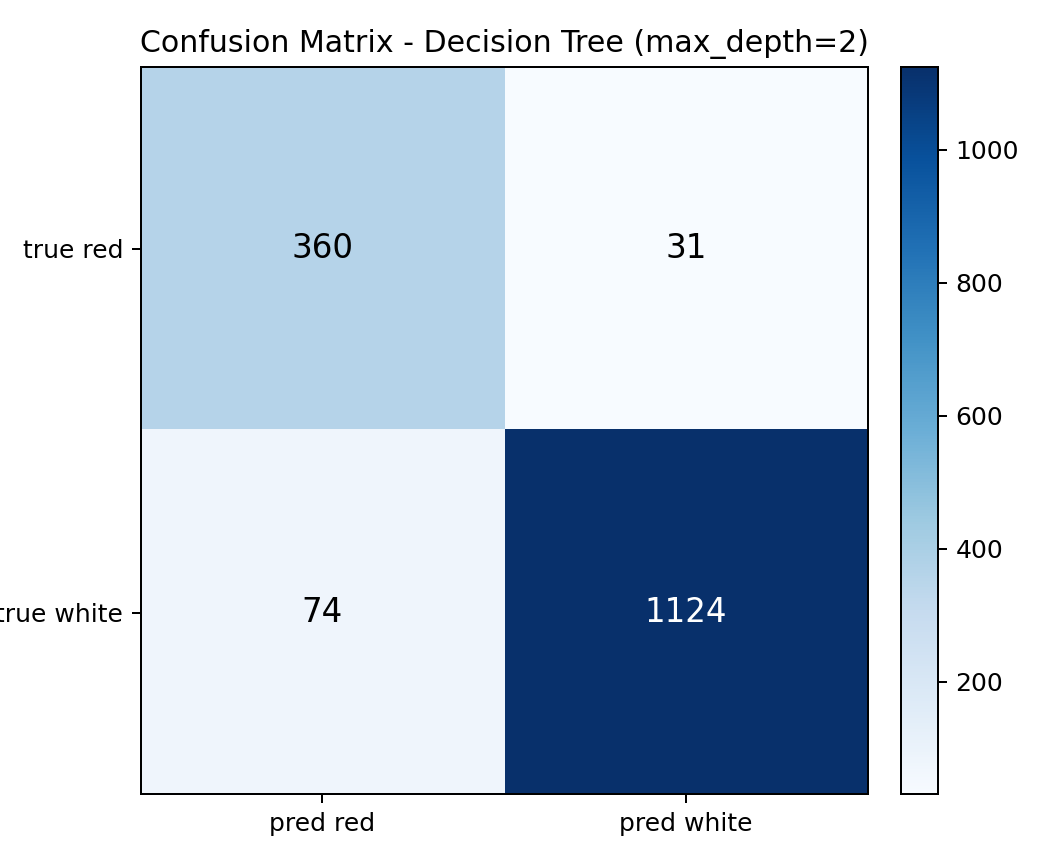
\includegraphics[width=0.62\textwidth]{q1_confusion_matrix.png}
\caption{Γραφική απεικόνιση του confusion matrix.}
\end{figure}

\subsection{Πώς διαβάζουμε τον confusion matrix}

Ο confusion matrix είναι ένας πίνακας που συγκρίνει τις πραγματικές κατηγορίες
με τις κατηγορίες που προέβλεψε το μοντέλο.

\begin{itemize}
    \item Το 360 σημαίνει ότι 360 κόκκινα κρασιά προβλέφθηκαν σωστά ως
    κόκκινα.
    \item Το 31 σημαίνει ότι 31 κόκκινα κρασιά προβλέφθηκαν λάθος ως λευκά.
    \item Το 74 σημαίνει ότι 74 λευκά κρασιά προβλέφθηκαν λάθος ως κόκκινα.
    \item Το 1124 σημαίνει ότι 1124 λευκά κρασιά προβλέφθηκαν σωστά ως λευκά.
\end{itemize}

Άρα το συνολικό πλήθος σωστών προβλέψεων είναι:

\[
    360 + 1124 = 1484.
\]

Το συνολικό πλήθος test παρατηρήσεων είναι:

\[
    360 + 31 + 74 + 1124 = 1589.
\]

Επομένως:

\[
    \text{Accuracy} = \frac{1484}{1589} = 0.9339.
\]

Τα συνολικά λάθη είναι:

\[
    31 + 74 = 105.
\]

Άρα:

\[
    \text{Test Error} = \frac{105}{1589} = 0.0661.
\]

%=============================================================================
\section{Οι κανόνες του δέντρου}
%=============================================================================

Ένα από τα μεγάλα πλεονεκτήματα των δέντρων ταξινόμησης είναι ότι μπορούμε να
δούμε τους κανόνες που χρησιμοποιούν. Το δικό μας δέντρο, επειδή έχει βάθος 2,
είναι αρκετά απλό.

\begin{figure}[H]
\centering
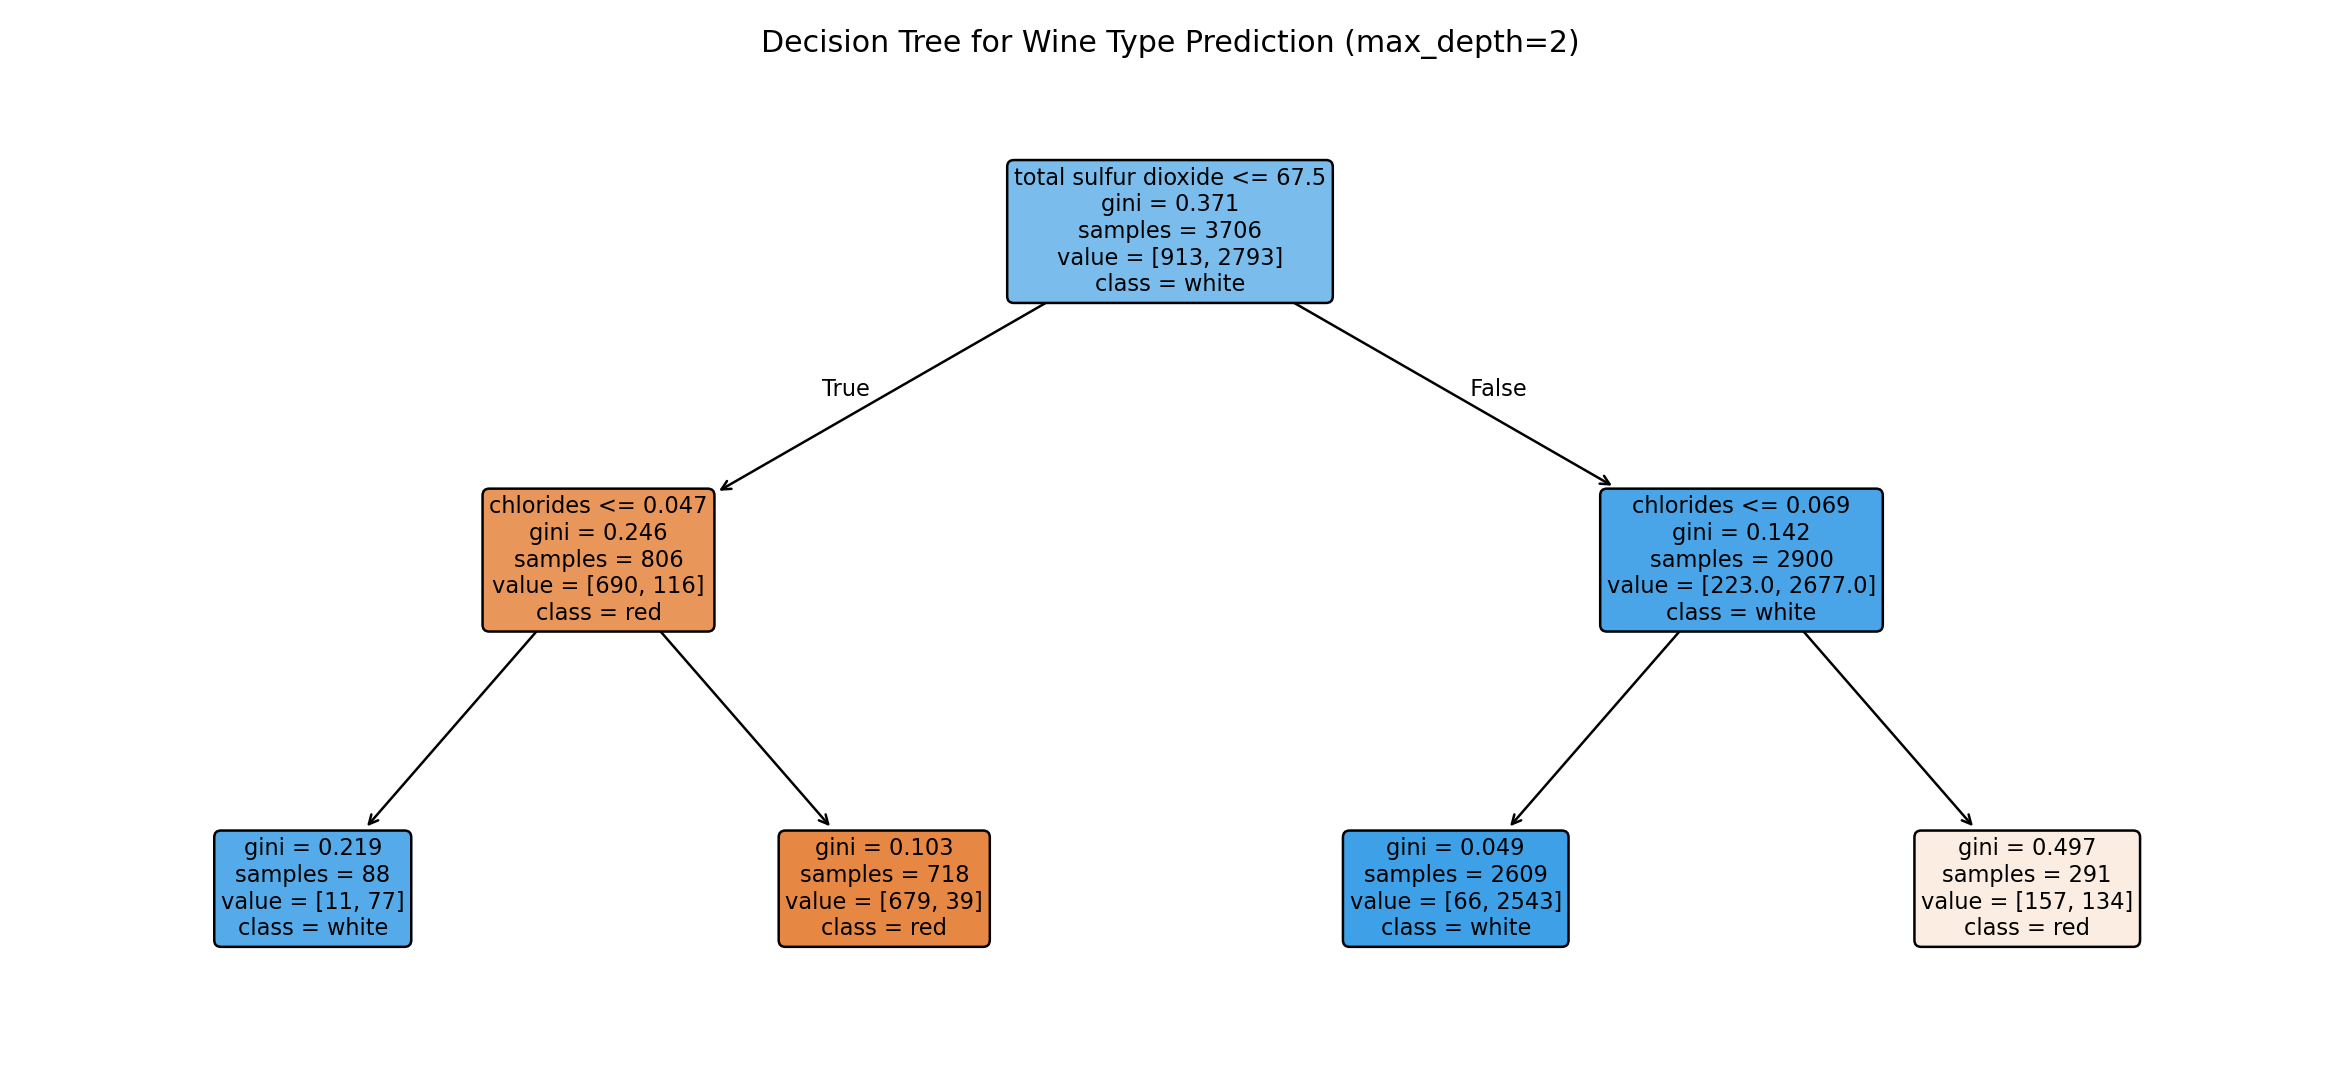
\includegraphics[width=\textwidth]{q1_decision_tree_plot.png}
\caption{Το δέντρο ταξινόμησης με \code{max\_depth=2}.}
\end{figure}

Οι κανόνες του δέντρου είναι:

\begin{verbatim}
total sulfur dioxide <= 67.50
|-- chlorides <= 0.05  -> white
|-- chlorides >  0.05  -> red

total sulfur dioxide > 67.50
|-- chlorides <= 0.07  -> white
|-- chlorides >  0.07  -> red
\end{verbatim}

\subsection{Ερμηνεία των κανόνων}

Το δέντρο χρησιμοποιεί κυρίως δύο μεταβλητές:

\begin{itemize}
    \item \code{total sulfur dioxide}
    \item \code{chlorides}
\end{itemize}

Η πρώτη ερώτηση που κάνει είναι:

\begin{quote}
Είναι το \code{total sulfur dioxide} μικρότερο ή ίσο από 67.50;
\end{quote}

Ανάλογα με την απάντηση, το δέντρο κοιτάζει μετά τη μεταβλητή
\code{chlorides}. Αν τα \code{chlorides} είναι χαμηλά, το δέντρο τείνει να
προβλέπει \code{white}. Αν είναι υψηλότερα, τείνει να προβλέπει \code{red}.

Με απλά λόγια, το δέντρο ανακάλυψε ότι οι μεταβλητές που σχετίζονται με τα
θειώδη και τα χλωριούχα άλατα βοηθούν πολύ στη διάκριση λευκού και κόκκινου
κρασιού.

\subsection{Γιατί αυτό είναι χρήσιμο}

Το αποτέλεσμα δεν είναι μόνο ένας αριθμός accuracy. Μας δίνει και μία απλή
ερμηνεία:

\begin{quote}
Ακόμη και με λίγους κανόνες, κάποια χημικά χαρακτηριστικά φαίνεται να
διαχωρίζουν αρκετά καλά τα λευκά από τα κόκκινα κρασιά.
\end{quote}

Αυτό είναι σημαντικό, γιατί ένα δέντρο ταξινόμησης δεν λειτουργεί σαν
«μαύρο κουτί» στον ίδιο βαθμό με άλλες μεθόδους. Μπορούμε να δούμε ποια
χαρακτηριστικά χρησιμοποίησε και πώς πήρε τις αποφάσεις του.

%=============================================================================
\section{Τελικός σχολιασμός για το Ερώτημα 1}
%=============================================================================

Το δέντρο ταξινόμησης μέγιστου βάθους 2 πέτυχε test accuracy 0.9339. Αυτό
είναι αρκετά υψηλή ακρίβεια, ειδικά αν λάβουμε υπόψη ότι το μοντέλο είναι
πολύ απλό.

Το βασικό συμπέρασμα είναι ότι ακόμη και ένα μικρό δέντρο, με λίγους μόνο
κανόνες, μπορεί να ταξινομήσει σωστά τα περισσότερα κρασιά ως λευκά ή κόκκινα.
Συγκεκριμένα, από τις 1589 παρατηρήσεις του test set, το μοντέλο ταξινόμησε
σωστά τις 1484 και έκανε λάθος στις 105.

Παρόλα αυτά, επειδή το δέντρο έχει περιορισμένο βάθος, δεν μπορεί να εκφράσει
πολύ σύνθετους κανόνες. Αυτό σημαίνει ότι υπάρχει πιθανότητα άλλα μοντέλα,
όπως Bagging, Random Forest ή Boosting, να πετύχουν ακόμη καλύτερη απόδοση.
Πράγματι, αυτό είναι κάτι που εξετάζεται στα επόμενα ερωτήματα της εργασίας.

\subsection{Σύντομη απάντηση που μπορεί να μπει στην εργασία}

Για το πρώτο ερώτημα εφαρμόστηκε δέντρο ταξινόμησης με μέγιστο βάθος
\code{max\_depth=2}. Ως προβλεπτικές μεταβλητές χρησιμοποιήθηκαν όλες οι
μεταβλητές εκτός από τη \code{quality} και τη \code{wine\_type}, ενώ η
\code{wine\_type} ήταν η μεταβλητή στόχος. Τα δεδομένα χωρίστηκαν σε training
set 70\% και test set 30\% με \code{random\_state=6931}. Το μοντέλο πέτυχε
test accuracy 0.9339 και test error 0.0661. Ο confusion matrix έδειξε ότι
ταξινομήθηκαν σωστά 360 κόκκινα και 1124 λευκά κρασιά, ενώ έγιναν 105 λάθη
συνολικά. Το δέντρο βασίστηκε κυρίως στις μεταβλητές \code{total sulfur dioxide}
και \code{chlorides}. Συμπερασματικά, ακόμη και ένα απλό δέντρο βάθους 2
παρέχει αρκετά καλή πρόβλεψη του τύπου κρασιού.

%=============================================================================
\appendix
\section{Αρχεία που δημιουργήθηκαν για το report}
%=============================================================================

Για το επεξηγηματικό report του Ερωτήματος 1 δημιουργήθηκαν τα παρακάτω
αρχεία:

\begin{itemize}
    \item \code{q1\_explanatory\_decision\_tree.py}: script που αναπαράγει τη
    λύση.
    \item \code{q1\_explanatory\_results.csv}: συγκεντρωτικός πίνακας
    αποτελεσμάτων.
    \item \code{q1\_class\_distribution.csv}: κατανομή των κλάσεων στο dataset.
    \item \code{q1\_tree\_rules.txt}: κανόνες του δέντρου σε μορφή κειμένου.
    \item \code{q1\_decision\_tree\_plot.png}: εικόνα του δέντρου.
    \item \code{q1\_confusion\_matrix.png}: εικόνα του confusion matrix.
    \item \code{explanatory\_report\_q1\_decision\_tree.tex}: το παρόν
    LaTeX αρχείο.
\end{itemize}

\end{document}
